\documentclass[a4paper,12pt]{article}
%spellchecker
% !TeX spellcheck = de

\usepackage{amssymb} % needed for math
\usepackage{amsmath} % needed for math
\usepackage[utf8]{inputenc} % this is needed for german umlauts
\usepackage[ngerman]{babel} % this is needed for german umlauts
\usepackage[T1]{fontenc}    % this is needed for correct output of umlauts in pdf
\usepackage[margin=2.5cm]{geometry} %layout
\usepackage{booktabs}

% this is needed for forms and links within the text
\usepackage{hyperref}  

% glossar, see http://en.wikibooks.org/wiki/LaTeX/Glossary
% has to be loaded AFTER hyperref so that entries are clickable
\usepackage[nonumberlist]{glossaries} 

% The following is needed in order to make the code compatible
% with both latex/dvips and pdflatex.
\ifx\pdftexversion\undefined
\usepackage[dvips]{graphicx}
\else
\usepackage[pdftex]{graphicx}
\DeclareGraphicsRule{*}{mps}{*}{}
\fi

\makeglossaries

%%%%%%%%%%%%%%%%%%%%%%%%%%%%%%%%%%%%%%%%%%%%%%%%%%%%%%%%%%%%%%%%%%%%%%
% Variablen                                 						 %
%%%%%%%%%%%%%%%%%%%%%%%%%%%%%%%%%%%%%%%%%%%%%%%%%%%%%%%%%%%%%%%%%%%%%%
\newcommand{\authorName}{Lena Gregor, Dominik Horn}
\newcommand{\auftraggeber}{Lehrstuhl für Datenbanksysteme}
\newcommand{\auftragnehmer}{Database Systems Studenten Team}
\newcommand{\projektName}{Wahlinformationssystem}
\newcommand{\tags}{\authorName, Lastenheft, TUM, Universität Augsburg, LMU}
\newcommand{\glossarName}{Glossar}
\title{\projektName~(Lastenheft)}
\author{\authorName}
\date{\today}

%%%%%%%%%%%%%%%%%%%%%%%%%%%%%%%%%%%%%%%%%%%%%%%%%%%%%%%%%%%%%%%%%%%%%%
% PDF Meta information                                 				 %
%%%%%%%%%%%%%%%%%%%%%%%%%%%%%%%%%%%%%%%%%%%%%%%%%%%%%%%%%%%%%%%%%%%%%%
\hypersetup{
  pdfauthor   = {\authorName},
  pdfkeywords = {\tags},
  pdftitle    = {\projektName~(Lastenheft)}
} 
 
%%%%%%%%%%%%%%%%%%%%%%%%%%%%%%%%%%%%%%%%%%%%%%%%%%%%%%%%%%%%%%%%%%%%%%
% Create a shorter version for tables. DO NOT CHANGE               	 %
%%%%%%%%%%%%%%%%%%%%%%%%%%%%%%%%%%%%%%%%%%%%%%%%%%%%%%%%%%%%%%%%%%%%%%
\newcommand\addrow[2]{#1 &#2\\ }

\newcommand\addheading[2]{#1 &#2\\ \hline}
\newcommand\tabularhead{\begin{tabular}{lp{13cm}}
\hline
}

\newcommand\addmulrow[2]{ \begin{minipage}[t][][t]{2.5cm}#1\end{minipage}% 
   &\begin{minipage}[t][][t]{8cm}
    \begin{enumerate} #2   \end{enumerate}
    \end{minipage}\\ }

\newenvironment{usecase}{\tabularhead}
{\hline\end{tabular}}

\usepackage{pdfpages}

%%%%%%%%%%%%%%%%%%%%%%%%%%%%%%%%%%%%%%%%%%%%%%%%%%%%%%%%%%%%%%%%%%%%%%
% THE DOCUMENT BEGINS             	                              	 %
%%%%%%%%%%%%%%%%%%%%%%%%%%%%%%%%%%%%%%%%%%%%%%%%%%%%%%%%%%%%%%%%%%%%%%
\begin{document}
 \pagenumbering{roman}
 \begin{titlepage}
\maketitle
\thispagestyle{empty} % no page number

\begin{verbatim}












\end{verbatim}


  \begin{tabular}[t]{ll}
	Projekt:       & \quad \projektName \\[1.2ex]
	Auftraggeber:  & \quad \auftraggeber\\[1.2ex]
	Auftragnehmer: & \quad \auftragnehmer\\[1.2ex]
  \end{tabular}

\begin{tabular}{|p{3 cm}|p{3 cm}|p{5 cm}|}
\hline
\textbf{Version} & \textbf{Datum} & \textbf{Autor(en)} \\
\hline
\hline
1.0 & 04.11.2019 & \authorName \\
\hline
\end{tabular}
\end{titlepage}
         % Deckblatt.tex laden und einfügen
 \setcounter{page}{2}
 \tableofcontents          % Inhaltsverzeichnis ausgeben
 \clearpage
 \pagenumbering{arabic}
 
\section{Zielbestimmung}
%%%%%%%%%%%%%%%%%%%%%%%%%%%%%%%%%%%%%%%%%%%%%%%%%%%%%%%%%%%%%%%%%%%%%%
% Warum wird das Projekt gemacht?           						 %
%%%%%%%%%%%%%%%%%%%%%%%%%%%%%%%%%%%%%%%%%%%%%%%%%%%%%%%%%%%%%%%%%%%%%%
Der Freistaat Bayern möchte in Kooperation mit dem Lehrstuhl für Datenbanksysteme an der Technischen Universität München
eine digitales Wahlinformations- und Stimmabgabesystem von Studierenden des Elite Software Engineering Masterstudiengangs 
für Landtagswahlen aufbauen.
Das System soll dabei nicht nur die Ergebnisse für die Landtagswahlen 2013 und 2018 analysierbar machen (Sitzverteilung im
Landtag, Vergleiche zwischen Wahlen, Zusammensetzung des Landtags) sondern auch als sicheres Backendsystem für die
elektronische Stimmabgabe im Wahllokal dienen. Es müssen die gesetzlichen Regelungen und Normen und Datenschutzaspekte
berücksichtigt werden. Als gesetzliche Basis dienen die Regelungen zur Landtagswahl 2018.

\section{Produkteinsatz}
%%%%%%%%%%%%%%%%%%%%%%%%%%%%%%%%%%%%%%%%%%%%%%%%%%%%%%%%%%%%%%%%%%%%%%
% Wer ist die Zielgruppe?                   						 %
%%%%%%%%%%%%%%%%%%%%%%%%%%%%%%%%%%%%%%%%%%%%%%%%%%%%%%%%%%%%%%%%%%%%%%
Zielgruppe ist im Wesentlichen der Übungsleiter der Database Systems Vorlesung
(Christian Winter) und die Studierenden/Entwickler. Konzipiert und Entwickelt
werden soll die Anwendung jedoch zur Verwendung durch Wahlhelfer zur 
Stimmeneintragung für Bayrische Landtagswahlen, zur Stimmabgabe durch Wahlberechtigte
(ggf. nach externer Personalverifikation durch Wahlhelfer) und zur (statistischen)-Auswertung
von Wahlergebnissen durch den oder die WahlleiterIn sowie u.U. interessierten BürgerInnen.

\section{Benutzerschnittstellen}
Die Informationsabfrage und (statistische) Auswertung von Wahlergebnissen erfolgt
in einer frei zugänglichen Weboberfläche. Hierbei soll auch der Vergleich zwischen verschiedenen
Wahlen möglich sein. Dafür muss es möglich sein, alte Wahlergebnisse in Form einer csv-Datei in das System einzulesen.  

Das Eintragen von einer oder mehreren Stimmabgaben ist als backend Aufruf (Serverless Function)
für authentifizierte Nutzer zugänglich. Diese Funktion machen sich Wahlhelfer oder Wahlleiter zunutze,
z.B. zum Übermitteln von Wahlergebnissen aus der jeweiligen Region.

Sämtliche Daten zu den Wahlen sollen in einem Datenbanksystem gespeichert werden.

Außerdem soll es möglich sein das System später als Backend für die elektronische Stimmabgabe im Wahllokal zu nutzen. Wie genau diese Schnittstelle aussehen soll, also ob die Stimmabgabe über eine Webseite oder ein lokales Programm erfolgen soll, wurde nicht vorgegeben.
 
%[<deckt sich so glaube ich nicht mit den Anforderungen auf dem Übungsblatt>
%Zur Einzelstimmabgabe im Wahllokal wird ebenfalls eine Weboberfläche zugänglich gemacht,
%die erst nach Freigabe durch eine(n) WahlhelferIn zur Abgabe von maximal einer Erststimme
%und einer Zweitstimme im jeweiligen Stimmkreis berechnet. Die vorangegangene Prüfung
%durch den Wahlhelfer stellt sicher, dass die Person wahlberechtigt ist und nicht bereits
%gewählt hat. Das System kann erweitert werden um den oder die WahlhelferIn beim
%Verifizierungsschritt zu unterstützen.]

\subsection{Auswertung von Wahlergebnissen}
\begin{center}
  \includegraphics{usecase.1}
\end{center}

\subsection{Eintragen von Wahlergebnissen durch Wahlhelfer}
\begin{center}
  \includegraphics{usecase.2}
\end{center}

\subsection{Stimmabgabe}
\begin{center}
  \includegraphics{usecase.3}
\end{center}

\section{Funktionale Anforderungen}
%%%%%%%%%%%%%%%%%%%%%%%%%%%%%%%%%%%%%%%%%%%%%%%%%%%%%%%%%%%%%%%%%%%%%%
% Was muss das Programm können?                   					 %
%%%%%%%%%%%%%%%%%%%%%%%%%%%%%%%%%%%%%%%%%%%%%%%%%%%%%%%%%%%%%%%%%%%%%%
\begin{usecase}
  \addheading{Nummer}{Beschreibung} 
  \addrow{FA01}{Wahldaten von Landtagswahlen ab (inklusive) 2013 müssen fehlerfrei aus einer csv-Datei importierbar und im System abbildbar sein}
  \addrow{FA02}{Das System muss in der Lage sein, als Backend für die Eingabe von Einzelstimmen durch Wahlberechtigte im Wahllokal zu fungieren (E-Voting). Die Verifizierung des Wahlberechtigten wird dabei durch die Wahlhelfer im Wahllokal vorgenommen. Das System muss also nicht über eine Verifizierungsmöglichkeit verfügen.}
  %{Einzelstimmen von Wahlberechtigen müssen über eine graphische Schnittstelle im Wahllokal eintragbar sein (E-Voting). 
              %  Hierbei muss gewährleistet sein, dass jede wahlberechtigte Person maximal eine Erst- und eine Zweitstimme abgeben darf.}
  \addrow{FA03}{Wahldaten müssen über eine graphische Schnittstelle (statistisch) auswertbar sein. Hierbei ist insbesondere das Bestimmen von
                Wahlergebnissen, d.h. gewonnenen Mandaten, wichtig.}
  \addrow{FA04}{Wahldaten unterschiedlicher Wahlvorgänge können verglichen werden.}
  \addrow{FA05}{Das System soll Einzelstimmen abspeichern können. Erst- und Zweitstimmen sollen getrennt voneinander abgespeichert werden.}
  \addrow{FA06}{Das System soll es erlauben, pro Stimmkreis die Einzelstimmen zu Stimmkreisergebnissen vorzuaggregieren.}
  \addrow{FA07}{Juristische Ausnahmefälle, die bei den Wahlen 2013 und 2018 nicht relevant waren und über Sperrklausel, Überhangsmandate, Ausgleichsmandate hinausgehen, müssen im System nicht verarbeitet/ berechnet werden können.}
  \addrow{FA09}{Das System muss in der Lage sein das Wahlergebnis einer Wahl zu berechnen und die statistische Auswertung laut Gesetzgebung (oder künftiger Spezifikation) bereit zu stellen.}
  
\end{usecase}

\section{Nichtfunktionale Anforderungen}
\begin{usecase}
  \addheading{Nummer}{Beschreibung} 
  \addrow{NF01}{Das System muss alle rechtlichen Vorgaben zur Landtagswahl im Freistaat Bayern einhalten, insbesondere im Bezug auf Datenschutz und Wahlgeheimnis.}
  \addrow{NF02}{Ein wirkungsvoller Schutz vor unbefugten Zugriffen muss ein fester Bestandteil sein.}
  \addrow{NF03}{Die graphische Oberfläche soll mächtig, jedoch intuitiv sein.}
\end{usecase}

\section{Produktdaten}
Verwaltete Produktdaten ergeben sich aus dem UML-Datenmodell auf der nächsten Seite:
%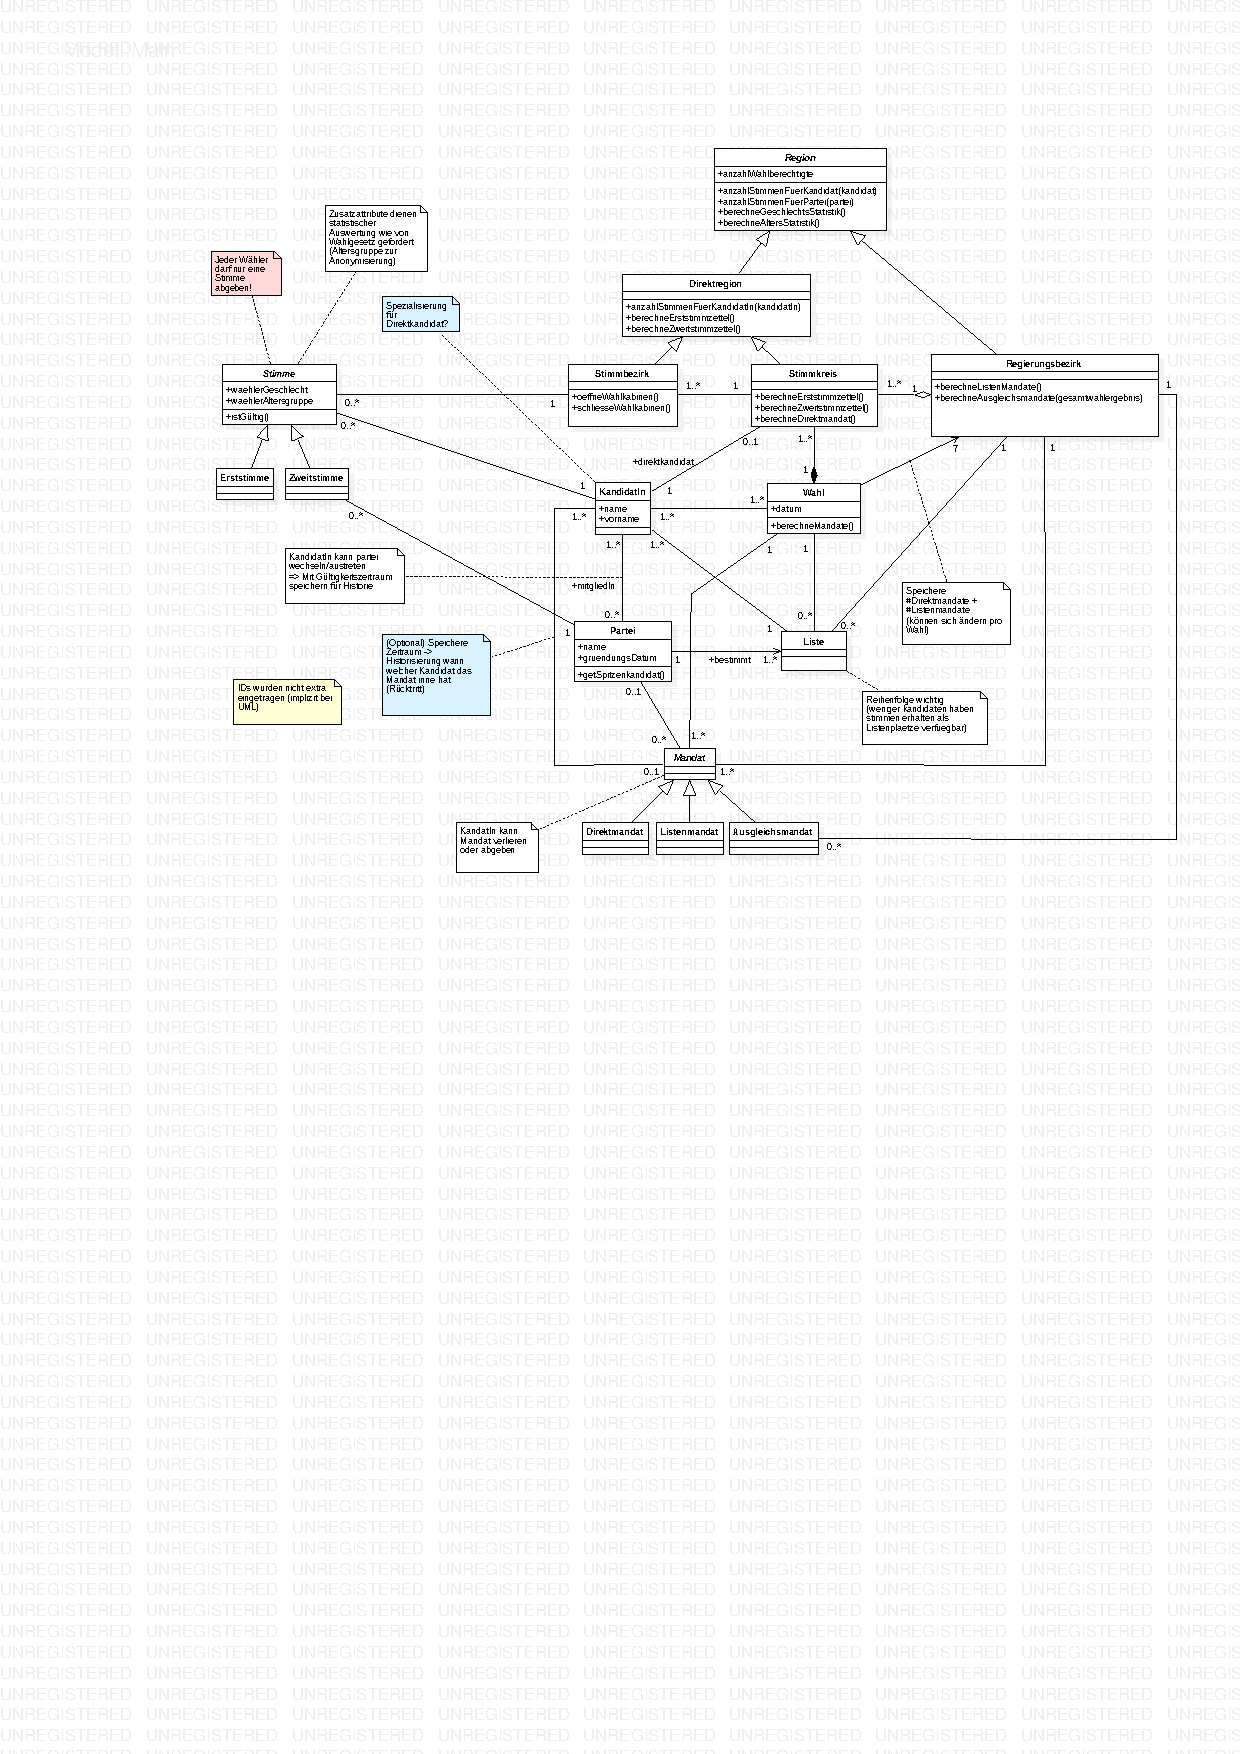
\includepdf[page={1}]{../model}

\begin{center}
	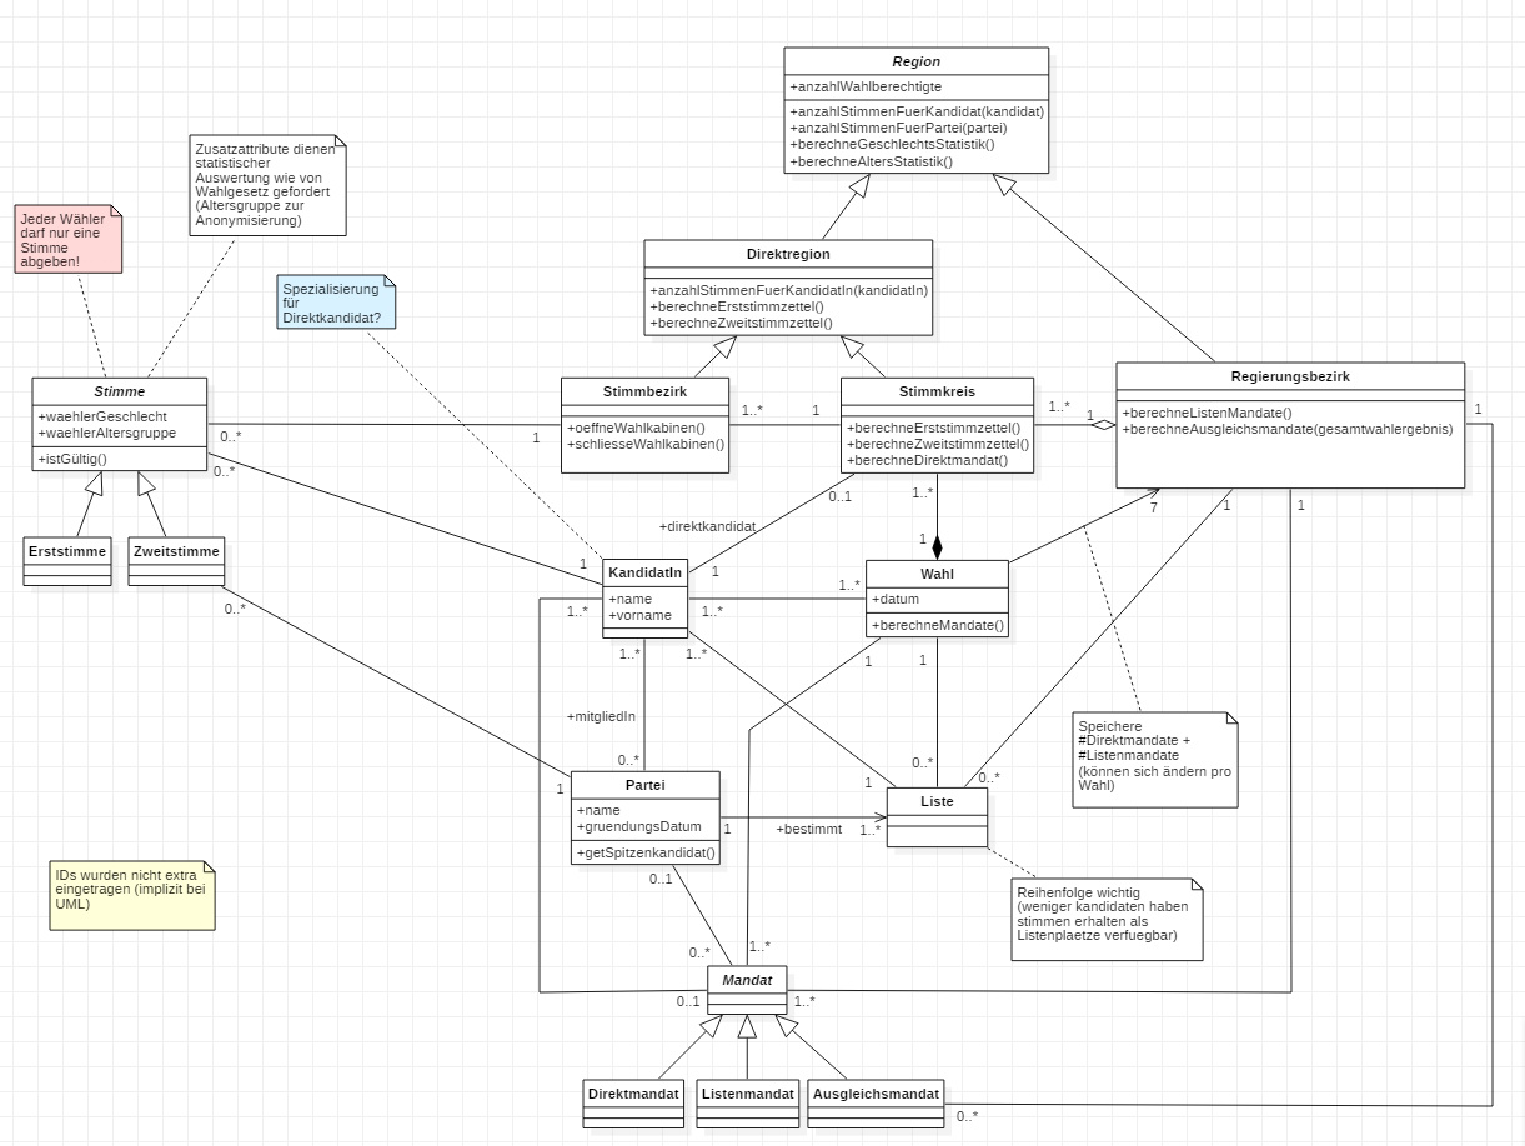
\includegraphics[width=\textwidth]{img/UML_Diagramm.pdf}
\end{center}

\section{Abnahmekriterien}
Das System erlaubt nach importieren von realen Stimmdaten deren (statistische) Auswertung, d.h. 
insbesondere die Bestimmung der gewonnenen Mandate im bayrischen Landtag. Dabei müssen gesetzliche
Vorgaben akkurat abgebildet sein sowie Daten sicher, Datenschutzrechtlich korrekt und integer gehalten
werden. Des weiteren sollte eine graphisch ansprechende Darstellung der (statistischen) Auswertung
einsehbar sein. 
%[Minimale Anforderung für den Einsatz im Wahllokal ist die Bereitstellung einer graphischen Schnittstelle zur Abgabe. von einzelnen Erst- und Zweitstimmen, welche unter Zuhilfenahme eines Wahlhelfers ausschließen können muss, dass die Wahlgesetzgebung verletzt wird. Diese Anforderung ist insbesondere im gesetzlichen Rahmen zur Stimmabgabe für bayrische Landtagswahlen zu verstehen.]

Für den Einsatz im Wahllokal ist die Bereitstellung einer Schnittstelle zum Systembackend notwendig. Die Schnittstelle soll später durch ein Frontend ergänzt werden können. Wichtig ist dafür, dass für jede Einzelstimme die Erst- und Zweitstimme getrennt gespeichert werden. 


% \clearpage
% %%%%%%%%%%%%%%%%%%%%%%%%%%%%%%%%%%%%%%%%%%%%%%%%%%%%%%%%%%%%%%%%%%%%%%
% Begriffslexikon zur Beschreibung des Produkts						 %
%%%%%%%%%%%%%%%%%%%%%%%%%%%%%%%%%%%%%%%%%%%%%%%%%%%%%%%%%%%%%%%%%%%%%%
%\newglossaryentry{sortierschluessel}
%{
%  name=Sortierschlüssel,
%  description={ein Schlüssel, anhand dessen diese Einträge sortiert werden}
%}
\newglossaryentry{Technologiestack}
{
  name=Technologiestack,
  description={Sammlung aller verwendeten Technologien im Projekt. Gegebenenfalls hierarchisch sortiert wenn aufeinander aufbauend}
}
\newglossaryentry{Client}
{
  name=Client,
  description={Programm, dass die Dienste eines Servers in Anspruch nimmt}
}
\newglossaryentry{Server}
{
  name=Server,
  description={Rechner, der für andere in einem Netzwerk mit ihm verbundene Systeme bestimmte Aufgaben übernimmt und von dem diese ganz oder teilweise abhängig sind}
}
\newglossaryentry{Datenbanksystem}
{
  name=Datenbanksystem,
  description={Ein Datenbanksystem (DBS) ist eine systematisch strukturierte, langfristig verfügbare Sammlung von Daten einschließlich der zur Verwaltung notwendigen Software}
}
\newglossaryentry{OLAP}
{
  name=OLAP,
  description={Online Analytical Processing}
}
\newglossaryentry{OLTP}
{
  name=OLTP,
  description={Online Transaction Processing}
}


% Setze den richtigen Namen für das Glossar
\renewcommand*{\glossaryname}{\section{\glossarName}}

% Drucke das gesamte Glossar
\glsaddall
\printglossaries

% Trage das Glossar in das Inhaltsverzeichnis ein
\stepcounter{section}
\addcontentsline{toc}{section}{\numberline {\thesection} \glossarName} 
\end{document}
